\documentclass[border=3mm,
tikz,margin=2cm]{standalone}
\usetikzlibrary{arrows.meta,
                calc, chains,
                quotes,
                positioning,
                shapes.geometric}


\begin{document}
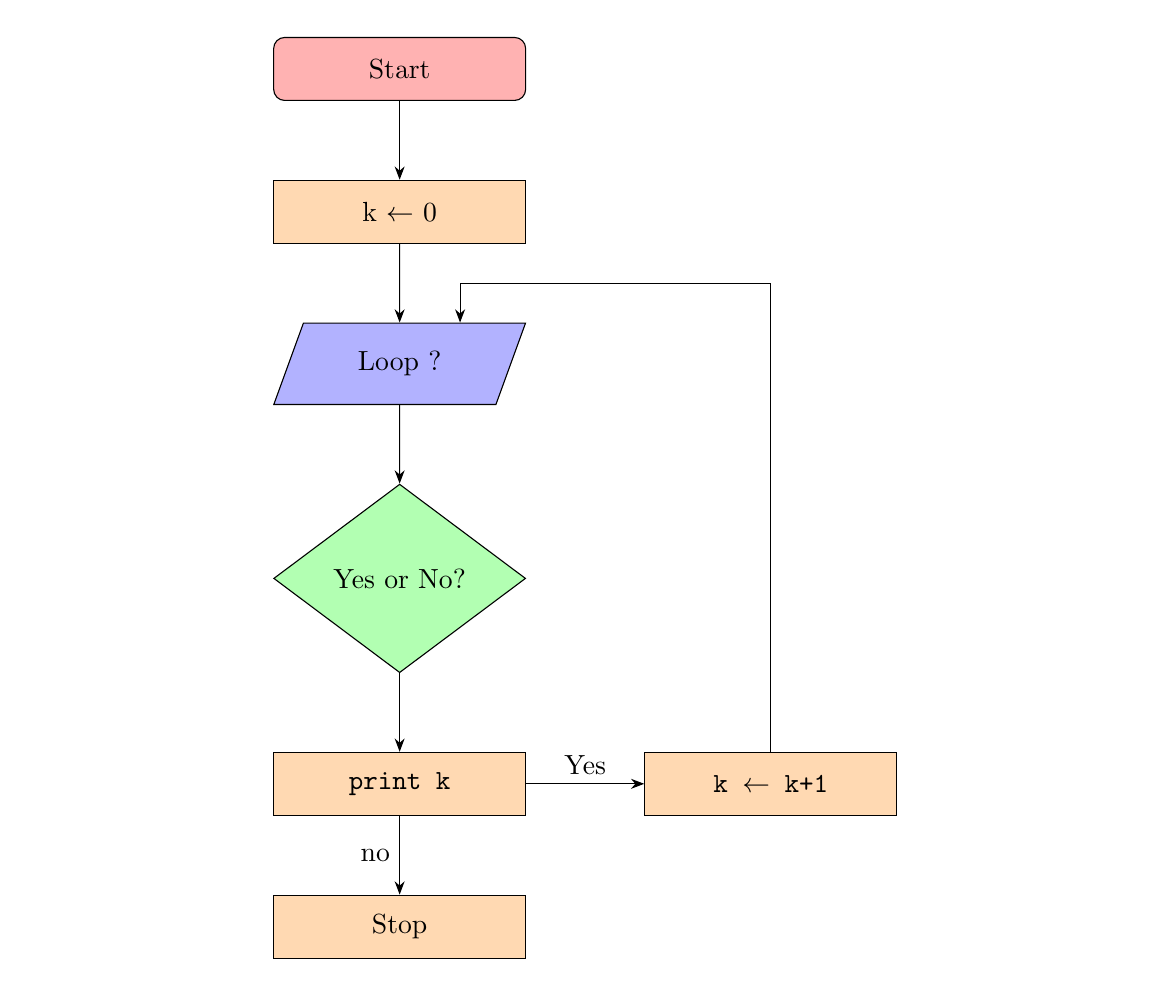
\begin{tikzpicture}[
    node distance = 8mm and 16mm,
        base/.style = {draw, minimum width=32mm, minimum height=8mm, align=center},
        startstop/.style = {base, rectangle, rounded corners, fill=red!30},
        process/.style = {base, rectangle, fill=orange!30},
        io/.style = {base, trapezium, 
                    trapezium left angle=70, trapezium right angle=110,
                    fill=blue!30},
        decision/.style = {base, diamond, fill=green!30},
        every edge quotes/.style = {auto=right},
        arrows=-Stealth
        ]

    \matrix[column sep=15mm, row sep=10mm]
    {
        % Row 1
        & & \node[startstop] (start) {Start}; & & &\\
        % Row 2
        & & \node[process] (k-0) {k $\leftarrow$ 0}; & & &\\
        % Row 3
        & & \node[io] (loop) {Loop ?}; & & &\\
        % Row 4
        & & \node[decision] (yesno) {Yes or No?}; & & &\\
        % Row 5
        &
        & \node[process] (printk) {\texttt{print k}};
        & \node[process] (k-kplus1) {\texttt{k $\leftarrow$ k+1}};
        & 
        &\\
        % Row 6
        & & \node[process] (stop) {Stop}; & & &\\
        % & & & & &\\
    };

    % 'edge' is used as new arrow is needed every time.
    % 'edge' is handled as a new path every time instead of one long path.
    \draw 
        (start)     edge        (k-0)
        (k-0)       edge        (loop)
        (loop)      edge        (yesno)
        (yesno)     edge        (printk)
        %% Branch
            (printk)    edge["Yes"']    (k-kplus1) % ending ' in "yes"' prints text on opposite side
            (k-kplus1)  |- ([xshift=3cm]$(loop.north)!0.5!(k-0.south)$) -| ([xshift=15mm]loop)
        %%
        (printk) edge["no"] (stop);

        
\end{tikzpicture}
\end{document}